% TeX file "regression_discontinuity_designs"

% Master thesis 
% Sven Jacobs
% Winter 2022, M.Sc. Economics, Bonn University
% Supervisor: Prof. Dr. Dominik Liebl


\section{Regression discontinuity designs}

We start with an overview of RD designs.
First, we formally introduce the so-called sharp design, where compliance with treatment assignment is perfect.
We then touch on departures from the standard sharp design.
Particularly the case of imperfect compliance, i.e.\ when treatment assignment and receipt do not coincide.
The remainder of the thesis, however, focuses on the sharp design.

\subsection{Sharp regression discontinuity design}

We assume to have a random sample of $n$ units, indexed by $i = 1, \dots, n$.
For each unit we observe $X_i$, the value of a continuous assignment variable $X$.
There exists a known cutoff $c$, such that units with $X_i \geq c$ are assigned to treatment.
Units with $X_i < c$ are assigned to the control group.
However, it is important to distinguish between being assigned to treatment and receiving treatment.
When some units do not comply with their assigned condition, we call this imperfect compliance.
In the sharp RD design such imperfect compliance is ruled out.
That is, all units assigned to the treatment group receive the treatment ($T = 1$), while all units assigned to the control group do not receive the treatment ($T = 0$).
As is shown in Figure~\ref{fig:treatment_probability_SRDD}, the conditional probability of receiving treatment $\Prob(T = 1 | X=x)$ therefore jumps \enquote{sharply} from zero to one at the cutoff.

To formalize treatment analysis, we employ the potential outcomes framework \parencite{Rubin_2005}.
The framework assumes that each unit has two potential outcomes, $Y_i(0)$ and $Y_i(1)$.
$Y_i(0)$ is the outcome that would be observed under control, and $Y_i(1)$ is the outcome that would be observed under treatment.
The fundamental problem of causal inference is that for each unit we only observe one outcome,
\begin{equation}
	Y_i = (1-T_i) \cdot Y_i(0) + T_i \cdot Y_i(1) = \begin{cases} 
		Y_i(0) & , X_i < c \\
		Y_i(1) & , X_i \geq c
	\end{cases} \,.
\end{equation}

\begin{figure}[p]
	\centering
	\begin{subfigure}{0.49\textwidth}
		\begin{tikzpicture}
			\begin{axis}
				[
				width=\textwidth,
				xlabel={Assignment variable, $X$}, xtick={0.5}, xticklabels={$c$}, 
				ylabel={Probability of receiving treatment}, ytick={0, 1}
				]
				
				\addplot[blue, mark=none]
				coordinates{(0, 0) (0.5, 0)};
				
				\addplot[red, mark=none]
				coordinates{(0.5, 1) (1, 1)};
				
				\addplot[blue, only marks, mark options={fill=white}]
				coordinates{(0.5, 0)};
				
				\addplot[red, only marks]
				coordinates{(0.5, 1)};
				
				\draw[dashed] (0.5, 0) -- (0.5, 1);	
			\end{axis}
		\end{tikzpicture}
		\caption{Sharp}
		\label{fig:treatment_probability_SRDD}
	\end{subfigure}
	\begin{subfigure}{0.49\textwidth}
		\begin{tikzpicture}
			\begin{axis}
				[
				width=\textwidth,
				xlabel={Assignment variable, $X$}, xtick={0.5}, xticklabels={$c$}, 
				ylabel={Probability of receiving treatment}, ytick={0, 1}
				]
				
				\addplot[blue, domain=0:0.5]
				expression{x^2};
				
				\addplot[red, domain=0.5:1]
				expression{-(x-1)^2 + 1};
				
				\addplot[blue, only marks, mark options={fill=white}]
				coordinates{(0.5, 0.25)};
				
				\addplot[red, only marks]
				coordinates{(0.5, 0.75)};
				
				\draw[dashed] (0.5, 0.25) -- (0.5, 0.75);	
			\end{axis}
		\end{tikzpicture}
		\caption{Fuzzy}
		\label{fig:treatment_probability_FRDD}
	\end{subfigure}
	\caption{Conditional probability of receiving treatment in RD designs.
			 Units to the left of the cutoff $c$ are assigned to control (in blue), units to the right to treatment (in red).}
	\label{fig:treatment_probability_RDD}
\end{figure}

\begin{figure}[p]
	\centering
	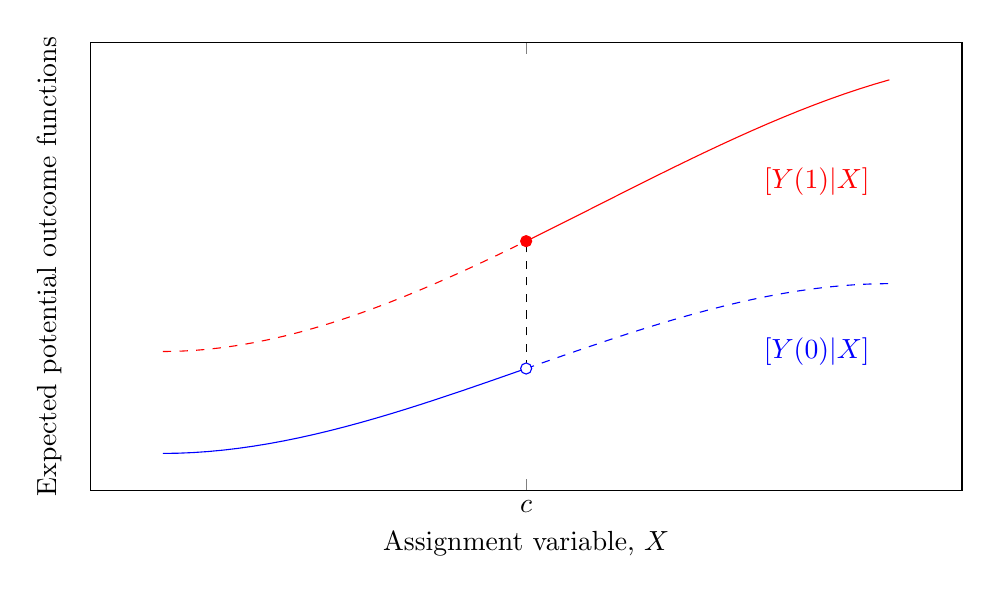
\begin{tikzpicture}
		\begin{axis}
			[
			width=1.5*240pt, height=207pt,
			xlabel={Assignment variable, $X$}, xtick={0.5}, xticklabels={$c$}, 
			ylabel={Expected potential outcome functions}, yticklabels={,,}, ytick style={draw=none} 
			]
			
			\addplot[blue, domain=0:0.5]
			expression{-0.5*x^3 + 0.75*x^2 + 0.3};
			
			\addplot[blue, dashed, domain=0.5:1]
			expression{-0.5*x^3 + 0.75*x^2 + 0.3};
			
			\addplot[red, domain=0.5:1]
			expression{-0.5*x^3 + 0.9*x^2 + 0.45};
			
			\addplot[red, dashed, domain=0:0.5]
			expression{-0.5*x^3 + 0.9*x^2 + 0.45};
			
			\addplot[blue, only marks, mark options={fill=white}]
			coordinates{(0.5, 0.425)};
			
			\addplot[red, only marks]
			coordinates{(0.5, 0.6125)};
			
			\draw[dashed] (0.5, 0.425) -- (0.5, 0.6125);
			
			\node[blue] at (axis cs:0.9, 0.45) {$\E[Y(0) | X]$};
			\node[red] at (axis cs:0.9, 0.7) {$\E[Y(1) | X]$};	
		\end{axis}
	\end{tikzpicture}
	\caption{Expected potential outcome function under control (in blue) and treatment (in red), respectively.
			 For units to the left of the cutoff $c$, we only observe control outcomes (according to the solid blue line) and no treatment outcomes (according to the dashed red line).
		 	 The opposite applies to units to the right of the cutoff.}
	\label{fig:regression_functions_SRDD}
\end{figure}
\noindent
Figure~\ref{fig:regression_functions_SRDD} illustrates this fundamental problem for the sharp design.
The figure shows two expected potential outcome functions, $\E[Y(0) | X=x]$ and $\E[Y(1) | X=x]$.
Both functions are plotted partly solid and partly dashed.
The reason is that in practice we can never observe realizations of the dashed function segments.
All units below the cutoff ($X_i < c$) are in the control group.
Thus, outcomes under treatment for this group are not observable (dashed red line).
All units above the cutoff ($X_i \geq c$) are treated.
Consequently, outcomes under control cannot be observed (dashed blue line).
Due to this lack of common support, the estimation of average (population) treatment effects, $\E[Y(1) - Y(0) | X = x]$, seems unfeasible.
In the next \hyperref[sec:identification]{section}, however, we state that under relatively mild conditions the average treatment effect (ATE) at the cutoff is identified in the sharp RD design.

\subsection{Fuzzy and other designs}  

In this thesis, we assume the basic RD setup, where all units comply with the treatment assignment (sharp design), there is one continuous assignment variable, and one cutoff.
In recent years, several extensions of the basic setup have been considered.
Especially, what is known as the fuzzy RD design.
In the fuzzy design there is still a discontinuity in the probability of receiving treatment at the cutoff, but not from zero to one.
The reason is imperfect compliance, i.e.\ some units assigned to control are treated, and/or some units supposed to be treated are not.
To give an example, in an early RD study, \textcite{Angrist_1999} investigate the effect of class size on scholastic achievement.
The authors exploit that primary schools in Israel are required to have no more than 40 pupils in a class.
Hence, at an enrollment-cutoff of 41, class size should drop sharply.
Some schools, however, still had classes with more than 40 pupils (e.g.\ due to scarcity of teachers), resulting in a fuzzy design.
An illustration of the conditional probability of being treated in a fuzzy design (with two-sided non-compliance) is depicted in Figure~\ref{fig:treatment_probability_FRDD}.
Such compliance issues hamper the treatment effect study, but many aspects from the sharp RD analysis carry over to the fuzzy case.
See, e.g., \textcite{Lee_2010}.

At this point, we just name a few other extensions.
The assignment variable can be discrete and have mass points \parencite{Kolesar_2018}.
A common example is age that is only available at an annual level.
RD designs can have multiple assignment variables \parencite{Papay_2011},
like two test scores (language and math).
A special case is the Geographic RD design, where treatment assignment changes at the border separating two areas.
Typically, latitude and longitude are then used for the analysis.
RD designs can also have multiple cutoffs but one assignment variable \parencite{Cattaneo_2016}.
For example, when regions choose a different cutoff to implement a federal program. 